\documentclass[a4paper,12pt,oneside]{article}

\usepackage{caption} 
\usepackage[T1]{fontenc} 
\usepackage[utf8]{inputenc} 
\usepackage{fancyhdr} 
\usepackage{lscape}

\usepackage{lmodern}

\usepackage[normalem]{ulem}
\usepackage[left=3cm,right=2cm,top=1.5cm,bottom=1cm,
textheight=245mm,textwidth=160mm,includeheadfoot,headsep=1cm,
footskip=1cm,headheight=14.599pt]{geometry}

\usepackage{graphicx} 
\usepackage{caption}
\usepackage{subcaption}
\usepackage{float}

\usepackage{epstopdf}

\usepackage{tabularx}
\usepackage{longtable}
\usepackage{multirow}

\usepackage{amsmath}
\usepackage{amsthm}
\usepackage{amssymb}
\usepackage{amsfonts}
\usepackage[shortlabels]{enumitem}


\theoremstyle{plain}
\newtheorem{thm}{Theorem}[section] % reset theorem numbering for each chapter

\theoremstyle{definition}
\newtheorem{defn}[thm]{Definition} % definition numbers are dependent on theorem numbers
\newtheorem{exmp}[thm]{Example} % same for example numbers
\theoremstyle{definition}

\newtheorem{subdefn}{Definition}[thm]
\renewcommand{\thesubdefn}{\thedefn\alph{subdefn}}

\newtheorem*{remark}{Remark}

\newcommand{\floor}[1]{\left\lfloor #1 \right\rfloor}
\newcommand{\ceil}[1]{\left\lceil #1 \right\rceil}

\usepackage{chngcntr}
\usepackage{apptools}
\AtAppendix{\counterwithin{lemma}{section}}
\AtAppendix{\counterwithin{theorem}{section}}

\newtheorem{theorem}{Theorem}[section]
\newtheorem{lemma}{Lemma}[section]
\newtheorem{corolarry}{Corolarry}[section]
\newtheorem{proposition}{Proposition}[section]
\newtheorem{claim}{Claim}[section]

\usepackage{setspace}
\onehalfspacing

\usepackage[colorlinks,pdfpagelabels,pdfstartview=FitH,
bookmarksopen=true,bookmarksnumbered=true,linkcolor=black,
plainpages=false,hypertexnames=false,citecolor=black]{hyperref}

\usepackage[backend=bibtex, style=numeric, bibstyle=numeric, maxcitenames=2]{biblatex}


 \bibliography{bib/literatur.bib}       

\usepackage{complexity}
\usepackage{eqparbox}
\usepackage{calligra}
\usepackage{rotating}

\usepackage{tikz-cd,tikz,tkz-graph,tkz-berge}
\usetikzlibrary{shapes.misc}
\usetikzlibrary{graphs}
\usetikzlibrary{graphs.standard}

\usepackage{epigraph}
\setlength\epigraphwidth{.8\textwidth}
\setlength\epigraphrule{0pt}

\usepackage{tikzscale}
\usetikzlibrary{decorations.pathreplacing}
\usetikzlibrary{arrows}

\usepackage{tkz-euclide}

\citetrackerfalse

\tikzcdset{every label/.append style = {font = \small}}
\usetikzlibrary{decorations.pathreplacing,angles,quotes}

\usepackage{pgfplots}
\usepgfplotslibrary{patchplots}
\usetikzlibrary{patterns, positioning, arrows}
\pgfplotsset{compat=1.15}

\usetikzlibrary{shapes.geometric}
\usetikzlibrary{positioning}

\usepackage[acronym]{glossaries}
\usepackage{pdfpages}

\usepackage{import}
\usepackage{pdfpages}
\usepackage{transparent}
\usepackage{xcolor}

\newcommand{\incfig}[2][1]{%
    \def\svgwidth{#1\columnwidth}
    \import{./figures/}{#2.pdf_tex}
}

\usepackage{titling}

\def\firstcircle{(90:1.75cm) circle (2.5cm)}
\def\secondcircle{(210:1.75cm) circle (2.5cm)}
\def\thirdcircle{(330:1.75cm) circle (2.5cm)}

\pdfsuppresswarningpagegroup=1

\title{Enumerative Combinatorics\\[0.3cm] \Large Lecture Notes}
\date{\today}
\author{David Scholz}

\begin{document}

\begin{titlingpage}
\maketitle
\end{titlingpage}

\newpage

\setcounter{page}{1} %Start the actually document on page 1

\thispagestyle{empty}
  
\newpage  
\pagestyle{empty}

\newpage

\begin{abstract}
    The following manuscript contains my lecture notes for the lecture "Introduction to Enumerative Combinatorics" by Prof. Evgeny Smirnov from HSE University. The following is taken directly 
    from the lecture unless otherwise noted. Sometimes we have expressed various ideas a little differently or filled them with more detailed information.
\end{abstract} 


\newpage
\pagestyle{empty}

\tableofcontents

\newpage
\pagestyle{fancy} 


\thispagestyle{empty}
\listoffigures

\newpage
\pagestyle{fancy}
\pagenumbering{arabic}
\section{Introduction}\label{introduction} 

We start by discussing fundamental combinatorial constructions such as words of a fixed alphabet, permutations of finite
sets and the number of subsets with a given number of elements. While we give some examples of how some combinatorial problems 
naturally arise, our main goal in this first section is to provide an intuitive introduction to the topic of 
Enumerative Combinatorics. 

\subsection{Words}

The first definition of this lecture is the definition of a word over a finite alphabet of symbols.

\begin{defn}[word]
Let $A$ be a finite set, called \textit{alphabet}. A \textit{word} is a finite sequence of elements of $A$. The \textit{size} of $A$ is its cardinality $|A|$.
The \textit{size} or \textit{length} of a word is its number of elements from $A$.
\end{defn}
\noindent
We might abuse language to a certain extent and call the elements of $A$ \textit{letters}.

\begin{exmp}
Let $A=\{1, 2, 3, 4\}$, then $112$, $132$, $1234$, $111$, $2345$, and so on are all words over $A$.
Notice that the length of the words is not fixed.    
\end{exmp}

In the study of combinatorics a very classical question is as follows. Given an alphabet $A$ of length $|A|=n$ , how many words over $A$ of length $k$ exist? This question leads us to the following theorem.

\begin{theorem}
The number of words of length $k$ in an alphabet consisting of $n$ letters is equal to $n^k$.
\label{thmNumWords}
\end{theorem}
\begin{proof}
There are $n$ possibilities for the first letter. The same holds for all other letters.
Thus, the total number of words equals
$$
\underbrace{n \cdot n \cdot n \cdots n}_\text{$k$-times} = n^k
$$
\end{proof}

The above proof is fairly simple, but there is a different possible interpretation of this problem. Let $X$ and $Y$ be sets. We might ask: what is the total
number of maps of the form $X \to Y$ without restrictions (an element in $Y$ can be hit multiple times)? It appears that this question can be solved using 
Theorem \ref{thmNumWords}. For seeing this, we number the elements of $X$ and $Y$ using natural numbers.
Given a map $f:X \to Y$, the sequence $f(1),f(2), \cdots, f(k)$ forms a word of length $k$. The number of words is therefore equivalent to the number of such maps.

\subsection{Permutations}

A notion that is closely related to the definition of a word, is the definition of a \textit{permutation}. First of all, the basic idea is to count maps, but 
usually with certain properties. Let $X$ and $Y$ be sets with $|X|=k$ and $|Y|=n$. We might ask: how many bijections $f:X \to Y$ are there? Recall that
a map is bijective if it is surjective and injective. In other words, given two elements $x,y \in X$ such that $f(x)=f(y)$, then it is implied that $x=y$ (the injective property), and 
every element of $Y$ appears in the preimage of a certain element of $X$ (the surjective property). It follows that the cardinalities of $X$ and $Y$ must be equal.
These observations lead us to the definition of a permutation.

\begin{defn}[permutation]
A \textit{permutation} is a bijection from $\{1, 2, 3, \cdots, n\}$ to itself.
\end{defn}
\noindent
In that sense the number of permutations is the number of bijections from $\{1, 2, \cdots, n\}$ to itself.
Equivalently, a permutation might be interpreted as a total linear ordering of the set $\{1, 2, 3, \cdots, n\}$.
If so, we need to arrange them in a certain way. How many ways to do this are there? 
The following theorem provides one possible solution.

\begin{theorem}
The number of permutations of $\{1, 2, \cdots, n\}$ is equal to $n!=1\cdot 2 \cdot 3 \cdots n$.\footnote{Recall that $0!=1$.}
\end{theorem}

\begin{proof}
There are $n$ choices for the first element. For the second element there are $n-1$ choices since
one element is already occupied. For the $k$-th element there are $n-k+1$ choices. For the last element there is one choice.
Thus, the total number of permutations is given by $n(n-1)(n-2)\cdots 2 \cdot 1=n!$. This completes the proof.
\end{proof}

In the following, we will generalize the above result to injective maps. Let $k \leq n$. In how many ways can we produce a collection 
of $k$ elements out of $n$? Such a collection is called a $k$-permutation.

\begin{defn}[$k$-permutation]
A $k$-permutation is a total linear ordering on a $k$-element subset of $\{1, 2, \cdots, n\}$.
\end{defn}

\begin{exmp}
Let $\{1,2 ,3\}$. A $1$-permutation is just a $1$-element subset, thus there is nothing order. The set of 
$2$-permutations is given by $\{\{1,2\}, \{1,3\}, \{2,1\}, \{2,3\}, \{3,1\}, \{3,2\}\}$.
Thus , there are six $2$-permutations in total.
\end{exmp}

\newpage

The general case of the number of $k$-permutations is examined in the following theorem.

\begin{theorem}
The number of $k$-permutations of $\{1,2, \cdots, n\}$ is equal to $$n(n-1)\cdots (n-k+1).$$
\end{theorem}

\begin{proof}
There are $n$ possible choices for the first entry of the subset. There are $(n-1)$ possible choices for the second element because the second element can occupy any entry except the one of the first element. 
For the $k$-th entry there are $n-k+1$ possible choices. All these possibilities are independent, hence
the total number of $k$-permutations is equal to their product $n(n-1)\cdots (n-k+1)$.
\end{proof}

The number $n(n-1)\cdots (n-k+1)$ is sometimes called the $k$ \textit{decreasing power} and is denoted by $n^{\downarrow k}$.

\subsection{Merry-go-rounds and Fermat's little theorem}

The problem which we are going to discuss next will illustrate a connection of combinatorics to algebra and number theory.

\subsection{Binomial coefficients}

Next, we consider the following important definition.

\begin{defn}[bionmial coefficient]
Let $k \leq n$. The number of $k$-element subsets of $\{1, 2, \cdots, n\}$ is called a \textit{binomial coefficient} ${n \choose k}$ ("$n$ choose $k$").
\end{defn}

How do we interpret this number? Suppose that we are hiring people to certain positions and suppose that we have $n$ candidates and we have $k$ identical positions.
The number of selecting $k$ people out of $n$ is called ${n \choose k}$. Notice that this is different than the problem from problem about $k$-permutations.
In our current case, the order of the $k$ elements that we choose does not matter. Thus, choosing all $k$ element subsets of a set and then ordering them in all possible ways
is equal to the $k$-permutations that we have seen above. How do we count the number of $k$-element subsets of a set?

\begin{theorem}
The number of $k$-element subsets of a set with cardinality $n$ is equal to 
$$
{n \choose k}=\frac{n!}{k!(n-k)!}=\frac{n(n-1)\cdots (n-k+1)}{k!}.
$$
\label{thmBinomial}
\end{theorem}

\begin{proof}
We consider ordered collections of distinct elements of length $k$. There are $n$ ways of choosing the first element, and $n-k+1$ ways of choosing the $k$-th element.
Hence there are 
$$
n(n-1)\cdots (n-k+1)=\frac{n!}{(n-k)!}
$$
ways such ordered collections. Since we are concerned with the number of unordered subsets and each subset has cardinality $k$, each subset can be rearranged in $k!$ ways.
Therefore, the number of ways to choose a $k$-element subset of a set with cardinality $n$ is given by 
$$
\frac{\frac{n!}{(n-k)!}}{k!}=\frac{n!}{k!(n-k)!}.
$$
This completes the proof.
\end{proof}

With the above theorem, we have shown something additionally that is not obvious at all and not necessarily easy to prove either.
We have also shown that the number $\frac{n(n-1)\cdots (n-k+1)}{k!}$ is integer.

At this point we provide some properties of binomial coefficients. We leave the proof as an easy exercise to the reader.

\begin{enumerate}[(i)]
    \item $\displaystyle {n \choose 0}={n \choose n}=1$.
    \item $\displaystyle {n \choose 1}={n \choose n-1}=n$
    \item $\displaystyle {n \choose 1}={n \choose n-k}$.
    \item $\displaystyle {n \choose k}={n - 1 \choose k -1} + {n - 1 \choose k}$.
\end{enumerate}

Let us examine property $(iv)$ in more detail. Despite its obvious algebraic proof, there is an intuitive combinatorial version as well.
We provide a proof sketch.

\begin{theorem}
$\displaystyle {n \choose k}={n - 1 \choose k -1} + {n - 1 \choose k}$
\label{recurrencePascal}
\end{theorem}

\begin{proof}[Proof-sketch]
Given a set $A=\{1, \cdots, n\}$ with $n$ elements. The number of $k$-element subsets of $A$ is ${n \choose k}$ according to theorem \ref{thmBinomial}.
Suppose that we pick the element $1$ of $A$, then all $k$-element subsets of $A$ are divided into two parts, some of them contain the element $1$, and the others do not.
Since we have already picked one element, we need to pick $k-1$ elements out of the remaining $n-1$ elements. There are ${n-1 \choose k-1}$ subsets containing $1$.
Thus, the subsets of cardinality $k$ that do not contain $1$ is equal to ${n - 1 \choose k}$, because we want to pick a $k$-element subset out of $n-1$ elements since $1$ element is forbidden.
\\
Adding up the two parts are equal to ${n \choose k}$. This completes the proof.
\end{proof}


\subsection{The Pascal triangle}

Binomial coefficients can be arranged in a triangle which is called the Pascal triangle.
Its rows are indexed by integers from $0$ up to infinity and in each row we write down all binomial coefficients.
For example, for ${n \choose k}$, $n=4$ represents the fifth row of the Pascal triangle and since $k \leq n$ there are $5$ binomial coefficients, namely ${4 \choose 0}=1, {4 \choose 1}=4, {4 \choose 2}=6, {4 \choose 3}=4$ and ${4 \choose 4}=1$.
\\
The relation given In Theorem \ref{recurrencePascal} provides a way of constructing the Pascal triangle. It says that the sum of two neighbors, namely ${n-1 \choose k-1}$ and ${n-1 \choose k}$ is equal to ${n \choose k}$. Thus, taking two neighbors in one row and
adding them up gives as the element below them (e.g. $3+3$ in row $n=3$ provides the element $6$ in the row $n=4$).
\\
\\
\begin{tabular}{>{$n=}l<{$\hspace{12pt}}*{13}{c}}
    0 &&&&&&&1&&&&&&\\
    1 &&&&&&1&&1&&&&&\\
    2 &&&&&1&&2&&1&&&&\\
    3 &&&&1&&3&&3&&1&&&\\
    4 &&&1&&4&&6&&4&&1&&\\
    5 &&1&&5&&10&&10&&5&&1&\\
    6 &1&&6&&15&&20&&15&&6&&1
\end{tabular}

\begin{proposition}
$\displaystyle {n \choose 0} + {n \choose k} + \cdots + {n \choose n}=2^n.$
\label{propositionPascalTriangle}
\end{proposition}

\begin{proof}
The binomial coefficient ${n \choose k}$ is the number of $k$-element subsets of a $n$-element set $A=\{1, \cdots, n\}$. Hence,
$$
\sum_{k=0}^n {n \choose k}
$$
is equal to the number of all possible subsets of $A$. We can associate a subset of $A$ with a binary number of length $n$ 
whereby each digit in this binary number represents a specific element in $A$. Now, setting a digit to $1$ means that we pick the element from $A$ at this position
for our subset. Setting it to $0$ means that we do not pick it. This is equal to the number of maps $\{1, \cdots, n\} \to \{0,1\}$ and the total number of such maps is equal to $2^n$ or in other words, the number of binary numbers that
can be represented with $n$ digits is equal to $2^n$. This completes the proof.
\end{proof}

We call the above binomial coefficients, because they arise as coefficients in the binomial formulas $(a+b)^n$. Let us prove this.

\begin{theorem}(Newton's Binomial Theorem)
$$
(a+b)^n = \sum_{k=0}^n {n \choose k} a^{n-k} \cdot b^k=a^n+n \cdot a^{n-1} \cdot b+ \frac{n(n-1)}{2} a^{n-2} \cdot b^2+ \cdots + n \cdot a \cdot b^{n-1}+b^n
$$
\label{newtonBinomialThm}
\end{theorem}

\begin{proof}
We expand the left-hand-side.
$$
(a+b)^n=\underbrace{(a+b)(a+b)(a+b)\cdots (a+b)}_{n-times}
$$
Every term in the above sum is the result of choosing either $a$ or $b$ from each of the $n$ factors. We want to calculate the coefficient for $a^{n-k}b^k$.
Since $b^k$, we must choose $b$ from exactly $k$ of the factors and we choose $a$ from the remaining $n-k$ factors.
Thus, the coefficients for $a^{n-k}b^k$ is equal to ${n \choose k}$. This completes the proof.
\end{proof}

\begin{corolarry}
$\displaystyle {n \choose 0}- {n \choose 1} + {n \choose 2} - {n \choose 3} + \cdots + (-1)^n {n \choose n}=0$
\end{corolarry}

\begin{proof}
Consider the binomial formula as provided in Theorem \ref{newtonBinomialThm}. Now, let $a=1$ and $b$ (or vice versa), it follows that 
$$
(1-1)^n= \sum (-1)^k {n \choose k}.
$$
\end{proof}

Notice, that Newton's binomial Theorem provides an easy proof for proposition \ref{propositionPascalTriangle} as well by considering $(1+1)^n=\sum {n \choose k}$.

\subsection{Exercises}

\begin{enumerate}
    \item Find the number of subsets of a $10$-element set with an odd number of elements.
    \item Compute the sum $\displaystyle \sum_{k=0}^n 2^k {n \choose k}$.
    \item Find the number of ways to rearrange the letters of the word \textit{EULER}.
    \item Find the number of ways to rearrange the letters of the word \textit{CATALAN}.
    \item How many necklaces can be formed with $7$ distinct beads? Necklaces can be rotated and/or flipped over. All beads must be used.
\end{enumerate}

\section[Permutations, binomial coefficients]{Permutations and binomial coefficients continued}\label{permutationsBinomialCoefficient} 

The following lecture discusses some more problems in which binomial coefficients arise and will lead us 
to the famous principle of exclusion and inclusion.

\subsection{The cab driver problem}

We will begin with the so called 'cab driver problem'. Suppose that we have a city with streets arranged in 
a regular grid (like Manhattan) and suppose that our city contains $n$ blocks from north to south and $m$ blocks
from west to east. Now, suppose that we have a cab driver that wants to drive from one point on the grid to another
point, say from $A$ to $B$. In figure \ref{fig:cabdriverprobleminitialexample} the general setup is visualized.

\begin{figure}[ht]
    \centering
    \scalebox{.6}{\incfig{cabdriverprobleminitialexample}}
    \caption{The Cap Driver Problem.}
    \label{fig:cabdriverprobleminitialexample}
\end{figure}
\noindent
\textbf{Question:} In how many ways can we get from $A$ to $B$? We are only allowed to go east or north and we are not allowed to go backwards.
\\
\\
Let $P_{m,n}$ be the number of paths from $A$ to $B$. We notice first, that we can solve this problem by considering a sequence of letters. Let 
us denote "going north" by the letter "N" and "going east" by the letter "E", then a path from $A$ to $B$ corresponds to a sequence of N's and E's
of length $m+n$ with $n$ N's and $m$ E's. The total number of such words is equal to the total number of paths from $A$ to $B$.
\\
\\
There is also another solution. Starting from any point in the above grid, there are only two choices: go north or go east. Let $A$ be the starting point
and denote "going north in the first step" by $A'$ and "going east in the second step" by $A''$, then the total number of paths from $A$ to $B$ is equal to 
the total number of paths from $A'$ to $B$ plus the total number of paths from $A''$ to $B$. The result is a so called recurrence relation given by the following equation.
$$
P_{A \to B}=P_{A' \to B} + P_{A'' \to B}
$$
In general, if we go one step north the first time, then there are $P_{m, n-1}$ paths left from this position to $B$. Similarly, if we go east first, then there are $P_{m-1, n}$
paths left from this position to $B$. This results in the following relation.
$$
P_{m, n}=P_{m,n-1}+P_{m-1, n}
$$
Given the initial conditions $P_{0,n}=P_{m,0}=1$, and $P_{m,1}=m+1$ and $P_{1,n}=n+1$, our final solution can be found quickly.
$$
P_{m,n}={m + n \choose m}={m+n \choose n}
$$

\subsection{Balls in boxes and multisets}

Suppose that we have $k$ balls and $n$ boxes. In how many ways can we put $k$ balls into $n$ boxes? If the maximal capacity of each box is $1$, the answer would be 
$n \choose k$ if $n \geq k$ and $0$ otherwise. What happens if there are no restrictions on the capacity of boxes?
\\
This question leads us to the definition of a multiset. Let $X$ be a set.

\begin{defn}
A multiset is a function $\mu: X \to \mathbb{Z}_{\geq  0}$. The size of a multiset is $\sum_{x \in X} \mu (x)$.
\end{defn}

\begin{exmp}
Assume that we have $5$ boxes, that is $X=\{1, 2, 3, 4 ,5\}$, and $\mu(1)=1, \mu(2)=0, \mu(3)=3$ and $\mu(4)=1$. Compare this with figure \ref{fig:multisetboxesexample}. Notice that box $3$ contains 
$3$ balls. The size of $\mu$ is $5$.

\begin{figure}[ht]
    \centering
    \scalebox{0.4}{\incfig{multisetboxesexamples3}}
    \caption{Balls in boxes and mutlisets.}
    \label{fig:multisetboxesexample}
\end{figure}
\end{exmp}

It is easy to see that the number of configurations of $k$ balls into $n$ boxes corresponds to the number of multisets of $\{1,2,\cdots, n\}$
of size $k$. Now, let us interpret our problem in a slightly different way. Imagine $k$ balls and separators (visualized as "$|$") that correspond to a box. Then, the above configuration configuration 
looks as follows.
$$
0\ |\ \ |\ 000\ |\ 0
$$
For $4$ boxes, we only need $3$ separators, or in general for $n$ boxes we need $n-1$ separators. Thus, configurations of balls in boxes correspond to configurations of bars and balls.
If we consider balls and bars to be objects, then we have $k+n-1$ objects in total.
\begin{tikzcd}
    & k \text{ balls}  \\
k+n-1 \arrow[ru] \arrow[rd] &                  \\
    & n-1 \text{ bars}
\end{tikzcd}

The above investigations encourage the following theorem.

\begin{theorem}
$k$ balls can be put into $n$ boxes in ${n+k-1 \choose k}$ ways. Equivalently, the number of $k$-element multisets in $\{1, \cdots, n\}$ is ${n+k-1 \choose k}$.
\end{theorem}
\noindent
The formal proof is left as an exercise for the reader.

\subsection{Integer compositions}

We are going to discuss integer compositions in the following section. We start with the formal definition.

\begin{defn}
An integer composition of $n \in \mathbb{Z}_{> 0}$ is a presentation of $n$ as  an ordered sum $n=n_1 + n_2 + \cdots + n_k, n_1,\cdots,n_k \in \mathbb{Z}_{> 0}$.
\end{defn}

\begin{exmp}
For $n=1$ there is only one trivial presentation, that is just $1$ itself. For $n=2$ there is one presentation, namely $2=1+1$. For $n=3$ there are $4$ presentations,
 namely $3=2+1=1+2=1+1+1$. Notice that this sums are ordered, thus $1+2$ and $2+1$ are considered to be different.
 For $n=4$ there are $8$ presentations, namely $4=3+1=1+3=2+2=2+1+1=1+2+1=1+1+2=1+1+1+1$.
\end{exmp}

\begin{theorem} The following statements are true.
\begin{enumerate}[(i)]
    \item The number of compositions of $n$ is $2^{n-1}$.
    \item The number of compositions of $n$ with exactly $k$ summands is ${n-1 \choose k-1}$.
\end{enumerate}
\end{theorem}

\begin{proof}
We start with $(ii)$. The composition of $n$ with exactly $k$ summands corresponds to configurations of $n$ balls 
inside $k$ boxes, s.t. each box is nonempty. This is the same as the number of configurations of $n-k$ balls in $k$ boxes, 
which is equal to
$$
{n-k+k-1 \choose k-1} = {n-1 \choose k-1}.
$$
We continue with $(i)$. The answer is trivial. The total number of compositions follows from the following equation.
$$
{n-1 \choose 0} + {n-1 \choose 1} + \cdots + {n-1 \choose n-1}=2^{n-1}.
$$
This completes the proof.
\end{proof}

\subsection{Principle of inclusion and exclusion}

In the following section we are going to introduce the "Principle of Inclusion and Exclusion (PIE)". Let us introduce this topic
with an example.

\begin{exmp}
Suppose that we have a room full of students. $25$ of them speak spanish, $24$ of them speak french and $8$ of them speak both spanish 
and french. How many students speak at least one foreign language? Denote the set of students speaking spanish by $S$ and the 
set of students speaking french by $F$. Now, consider the following Venn-diagram.
\begin{figure}[H]
    \centering
    \scalebox{0.6}{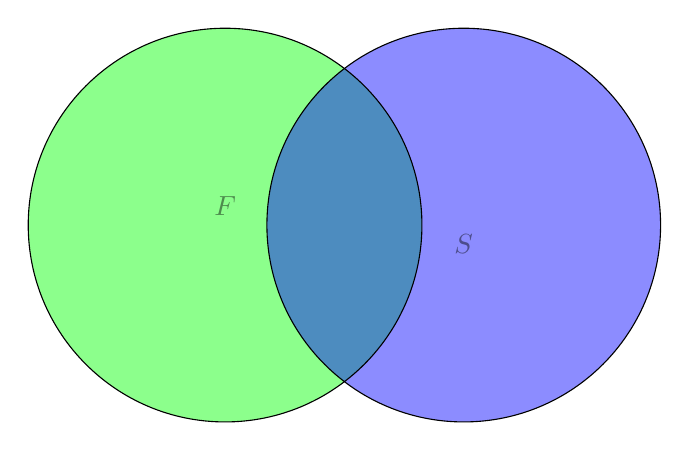
\begin{tikzpicture}
        \begin{scope}[shift={(3cm,-5cm)}, fill opacity=0.45]
            \fill[green] \secondcircle;
            \fill[blue] \thirdcircle;
            \draw \secondcircle node [above] {$F$};
            \draw \thirdcircle node [below] {$S$};
        \end{scope}
    \end{tikzpicture}}
    \caption{Venn-diagram for two languages.}
\end{figure}

The number of students that speak at least one language is equal to $|S \cup F|=|S| + |F|-|S \cap F|=25+24-8=41$. Notice that we must substract their intersection 
or we count the students speaking both french and spanish twice.\\\\
Now, suppose that $15$ students speak german, $6$ speak german and spanish, $7$ speak german and french and 
$4$ speak all three languages. Let us denote the set of students who speak german by $G$, the set of students who speak french by $F$ 
and the set of students that speak spanish by $S$. Consider the following Venn-diagram.

\begin{figure}[H]
    \centering
    \scalebox{0.6}{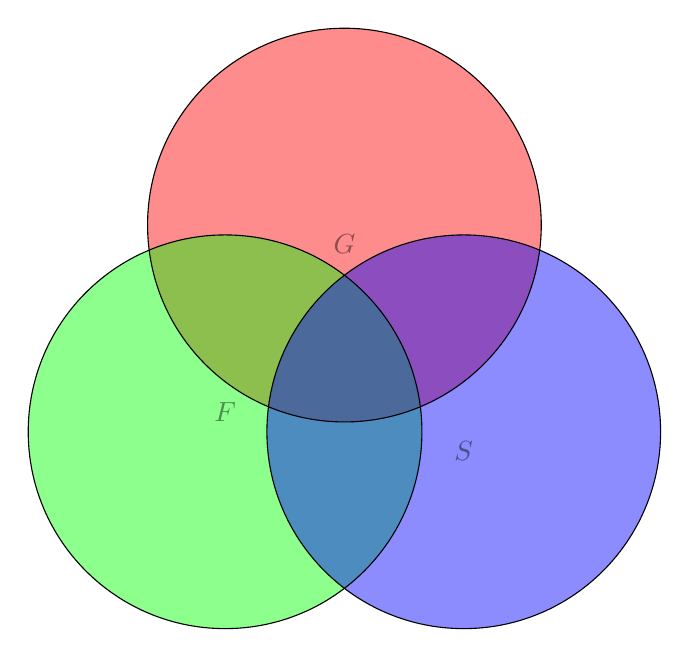
\begin{tikzpicture}
        \begin{scope}[shift={(3cm,-5cm)}, fill opacity=0.45]
            \fill[red] \firstcircle;
            \fill[green] \secondcircle;
            \fill[blue] \thirdcircle;
            \draw \firstcircle node[below] {$G$};
            \draw \secondcircle node [above] {$F$};
            \draw \thirdcircle node [below] {$S$};
        \end{scope}
    \end{tikzpicture}}
    \caption{Venn-diagram for three languages.}
\end{figure}
Now the result is very similar to the one before. The number of students that speak at least one language is equal to the following.
$$
|G \cup S \cup F|=|G| + |F| + |S| - |S \cap F| - |S \cap G| - |G \cap F| + |S \cap F \cap G|=25+24+15-8-7-6+4=47.
$$
\end{exmp}

Let us generalize this by the following theorem.

\begin{theorem}(Principle of inclusion-exclusion)
Let $A_1\cdots, A_n$ be finite subsets of a set $X$. Then 
\begin{align*}
|A_1 \cup \cdots \cup A_n|&=|A_1|+\cdots+|A_n|\\
&=\sum_{1 \leq i < j \leq n} |A_i \cap A_j|+\sum_{1 \leq i < j \leq n} |A_i \cap A_j \cap A_k| - \cdots + (-1)^{n-1}|A_1 \cap \cdots \cap A_n|.
\end{align*}
\end{theorem}

\begin{proof}
Let $x \in A_1 \cup \cdots \cup A_n$. How many times does $x$ appear on the right-hand-side? Suppose that $x \in A_1 \cap \cdots \cap A_p$ and 
$x \notin A_{p+1}, A_{p+2}, \cdots, A_n$. Then $x$ contributes to the right-hand-side with multiplicity 
$$
p- {p \choose 2} + {p \choose 3} - {p \choose 4} + \cdots + (-1)^{p-1} {p \choose p}=1+(-1 +p- {p \choose 2} + {p \choose 3} - \cdots + (-1)^{p-1} {p \choose p})=1.
$$
\end{proof}

The standard proof of the above is via induction. This is left as an exercise for the reader.

\subsection{The derangement problem}

\subsection{Exercises}

\begin{enumerate}
    \item Find the number of lattice paths from $(-2, -2)$ to $(3,3)$ passing through the point $(0,0)$ (each segment of a path goes north or east).
    \item In how many ways is it possible to permute the letters in the word \textit{EUCLID} in such a way that the order of the vowels (\textit{E,U,I}) is unchanged?
    \item Find the number of merry-go-rounds formed by $10$ carriages of two different colours.
    \item Find the number of positive integers not exceeding $300$ and \textbf{not} divisible by any of $2,3,$ and $5$.
\end{enumerate}

\section[Linear recurrences]{Linear recurrences - The Fibonacci sequence}\label{fibonacci} 

We are going to discuss the Fibonacci sequence in the following section.

\subsection{Fibonacci's rabbit problem}

Suppose we have a pair of rabbits that are adults after one month. In the month after they are fully grown,
they give birth to two more rabbits. The newborns are again fully grown after one month and give birth to two more 
rabbits, and so on. Consider the following figure as an example.
\\
\\
$
\begin{array}{l}
    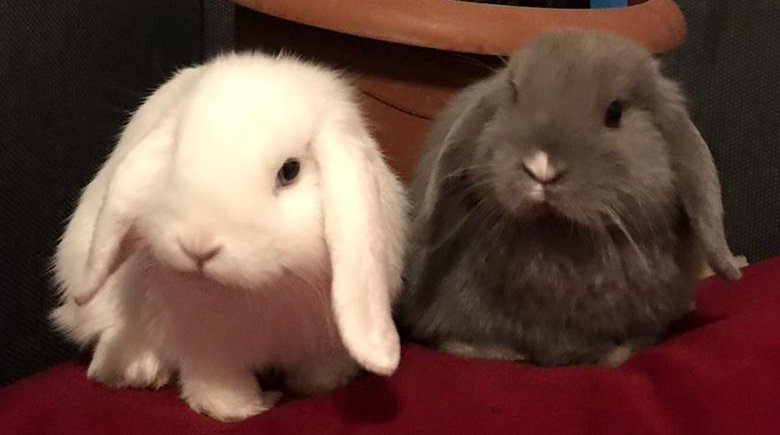
\includegraphics[scale=0.1]{pictures/rabbits.jpg}
\end{array}
n=1$\\
$
\begin{array}{l}
    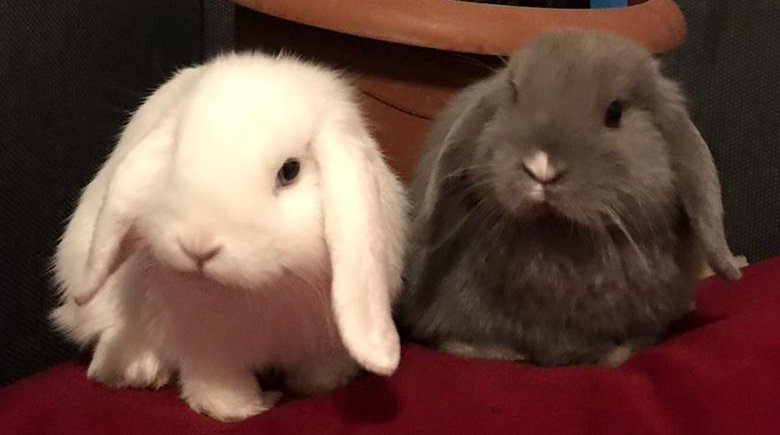
\includegraphics[scale=0.1]{pictures/rabbits.jpg}
\end{array}
n=2 \text{ (grown up)}$
\\
$
\begin{array}{l}
    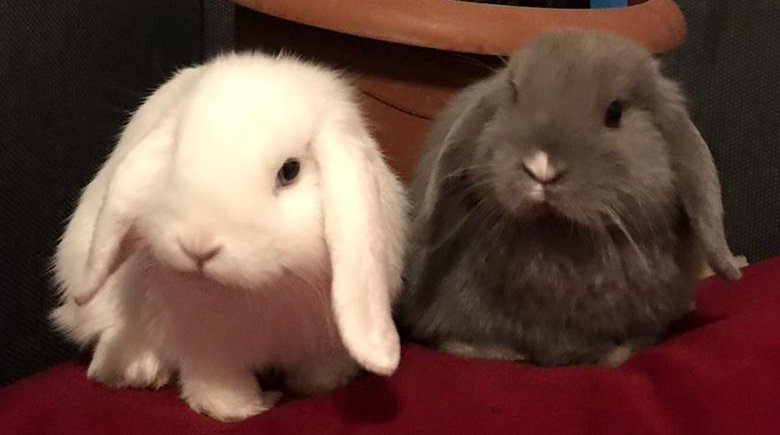
\includegraphics[scale=0.1]{pictures/rabbits.jpg}
    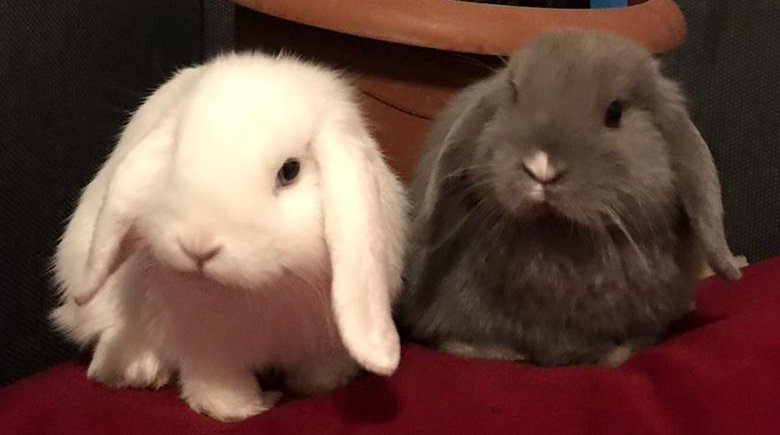
\includegraphics[scale=0.1]{pictures/rabbits.jpg}
\end{array}
n=3$
\\
$
\begin{array}{l}
    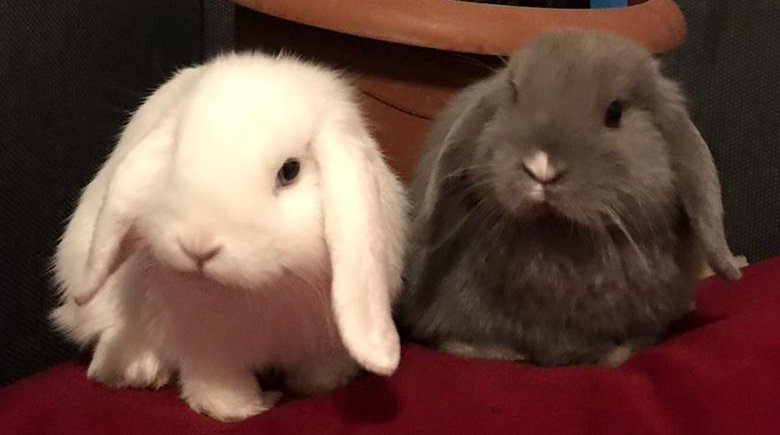
\includegraphics[scale=0.1]{pictures/rabbits.jpg}
    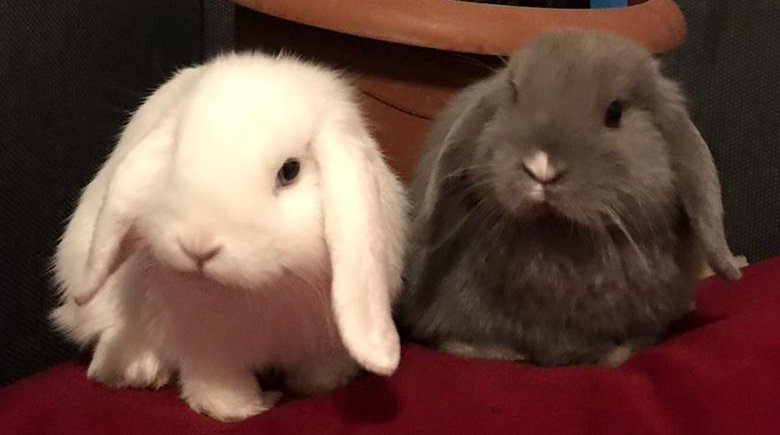
\includegraphics[scale=0.1]{pictures/rabbits.jpg}
    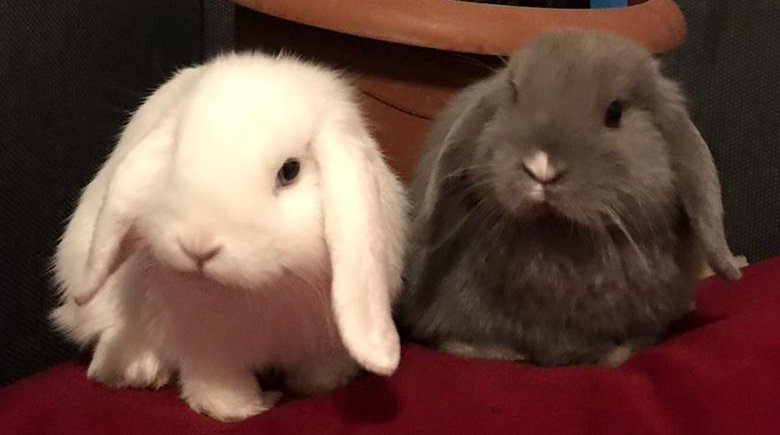
\includegraphics[scale=0.1]{pictures/rabbits.jpg}
\end{array}
n=4$
\\
\\
\noindent
\textbf{Question:} How many pairs of rabbits will we have after one year?
\\
\\
\noindent
Let us introduce the following notation. Denote the number of pairs of rabbits during
the $n$-th month by $F(n)$. Then, we could express $F(n)$ by the number of rabbits in 
the $(n-1)$-th month and $(n-2)$-th month by the following equation.
$$
F(n)=F(n-1)+F(n-2)
$$
Thus, by setting $F(2)=1$ the following sequence of numbers follows.
$$
1,1,2,3,5,8,13,21,36,55,89,144, \cdots
$$
\noindent
The answer follows for $F(12)=144$, hence after $12$ months we have $144$ pairs of rabbits.
\\
\\
The above sequence is called the "Fibonacci sequence" and we are going to investigate some 
of its fascinating properties in the next sections.

\newpage

\subsection[Pascal triangle]{Fibonacci numbers and the Pascal triangle}

We consider once again the Pascal triangle. Let us sum up its diagonals. This is done in the following figure for 
the first few diagonals.
\\
\\
\begin{tabular}{>{$n=}l<{$\hspace{12pt}}*{13}{c}}
    0 &&&&&&&1&&&&&&\\
    1 &&&&&&1&&\color{red}1\textsuperscript{\color{red}=2}&&&&&\\
    2 &&&&&\color{red}1&&\color{yellow}2\textsuperscript{\color{yellow}=3}&&1&&&&\\
    3 &&&&\color{yellow}1&&\color{green}3\textsuperscript{\color{green}=4}&&\color{blue}3\textsuperscript{\color{blue}=8}&&\color{cyan}1\textsuperscript{\color{cyan}=13}&&&\\
    4 &&&\color{green}1&&\color{blue}4&&\color{cyan}6&&4&&1&&\\
    5 &&\color{blue}1&&\color{cyan}5&&10&&10&&5&&1&\\
    6 &\color{cyan}1&&6&&15&&20&&15&&6&&1
\end{tabular}
\\
\\
\noindent
The following sequence is the result.
$$
1,1,
\color{red} 1 \color{black}+ \color{red}1\color{black}=\color{red}2 \color{black}, \color{yellow} 1 \color{black}+ \color{yellow}2\color{black}=\color{yellow}3 \color{black}, 
\color{green} 1 \color{black}+ \color{green}3\color{black}=\color{green}4 \color{black}, 
\color{blue} 1 \color{black}+ \color{blue}4\color{black}+ \color{blue}3=\color{blue}8 \color{black}, 
\color{cyan} 1 \color{black}+ \color{cyan}5\color{black}+ \color{cyan}6\color{black}+ \color{cyan}1=\color{cyan}13 \color{black}, \cdots 
$$
The general formula for the sum of the diagonals in the Pascal triangle is easily derived. It is as follows.
$$
\sum_{k=0}^{\floor{\frac{n-1}{2}}} {n-k-1 \choose k}
$$

\subsection{Domino tilings}

\subsection{Linear recurrence relations}

In the following section, we are going to introduce the formal definition of a linear recurrence relation.

\begin{defn}
A linear recurrence relation of order $k$ is a sequence satisfying 
$$
A(n)=c_1A(n-1)+c_2A(n-2)+\cdots+c_kA(n-k)
$$
where $c_1,\cdots, c_k \in \mathbb{R}$.
\label{defn:rec}
\end{defn}

\begin{exmp}
The Fibonacci sequence $F(n)=F(n-1)+F(n-2)$ is a linear recurrence relation of order $2$. The sequence
$A(n)=A(n-1)+A(n-2)+A(n-5)$ from the last section is a linear recurrence relation of order $5$.
\end{exmp}

\begin{remark}
A sequence defined by a linear recurrence relation is uniquely determined by the first $k$ terms $A(0), A(1), \cdots, A(k-1)$.
Why is that the case? Suppose that $a_0, a_1, a_2, \cdots$ and $a_0', a_1', a_2', \cdots$ satisfy the relation $(*)$,
then $a_0+a_0', a_1+a_1',a_2+a_2', \cdots$ also satisfy $(*)$ and so does $c \cdots a_0, c \cdot a_1, c \cdot a_2, \cdots$.
In other words, the solutions of a linear recurrence relation form a vector space.
\end{remark}

\subsection[The characteristic equation]{The characteristic equation}

In the following section we want to solve the following problem.\\
\textbf{Problem:} Given a recurrence relation
$$
(*)\ A(n)=c_1A(n-1)+c_2A(n-2)+\cdots+c_kA(n-k)
$$
as in definition \ref{defn:rec}. Find \underline{all} the sequences $(a_0, a_1, a_2, \cdots)$ satisfying this relation.
\\
For $k=1$ the linear recurrence relation yields $A(n)=c \cdot A(n-1)$, and the answer for our problem is just the geometric progression 
given by $a_n=c^n a_0$ where $a_0 \in \mathbb{R}$.
\\
\\
\noindent
\textbf{Idea:} Find a geometric progression $(a_0, \lambda a_0, \lambda^2 a_0, \cdots)$ satisfying $(*)$. Suppose $\lambda \neq 0$ and $a_0 \neq 0$.
Then,
$$
a_0 \lambda^n=c_1 a_0 \lambda^{n-1}+c_2 a_0 \lambda^{n-2} + \cdots + c_k a_0 \lambda^{n-k}, \forall n \geq k.
$$
Dividing the above equation by $a_0 \lambda^{n-k}$ yields 
$$
\lambda^k=c_1 \lambda^{k-1} + c_2 \lambda^{k-2} + \cdots + c_k.
$$
Then $\lambda$ is a root of the so called \underline{characteristic equation} which is given by
$$
t^k=c_1t^{k-1}+c_2 t^{k-2} + \cdots + c_k.
$$
The coefficients of the characteristic equation are the same as in the original recurrence relation.

\subsection{Linear recurrence relations of order $2$}

\subsection{The Binet formula}

\subsection{Linear recurrence relations of arbitrary order}

\subsection{The case of roots with multiplicities}

\subsection{Exercises}

\begin{enumerate}
\item Which of the following is a Fibonacci sequence?
\begin{enumerate}
\item The number of partitions, i.e. the presentations of a natural number as a sum of positive non-increasing summands (i.e., $3=2+1=1+1+1$)
\item The number of sequences of $0$'s and $1$'1 with $n$ digits that contain no two consecutive zeroes
\item The number of subsets of $\{1,2, \cdots, n\}$ that contain no consecutive integers
\item The number of partitions of a rectangle $2 \times n$ into rectangles $2 \times 1$
\item The number of compositions of a natural number into positive odd summands (i.e., $4=1+1+1+1=1+3=3+1$)
\end{enumerate}
\item The Fibonacci sequence can be continues "backwards" using the same rule: $F_n=F_{n-1}+F_{n-2}$. For example, $F_0=0, F_{-1}=1$. Find $F_{-10}$.
\item Find the maximal common ration of a geometric progression $a_n$ satisfying the following equation: $a_{n+2}=3a_{n+1}-2a_n$.
\item The sequence $a_n$ is defined by the recurrence relation $a_{n+3}=3a_{n+2}-3a_{n+1}+a_n$ with initial values $a_0=a_1=0, a_2=1$. Find $a_{100}$.
\item The sequence $a_n$ is defined by the recurrence relation $a_{n+4}=a_{n+3}-a_{n+2}+a_{n+1}-a_n$ with initial values $a_0=1607, a_1=1707, a_2=1814, a_3=1914$. Find $a_{100}$.
\end{enumerate}

\section{A nonlinear recurrence: many faces of Catalan numbers}\label{catalan} 

Hallo

\subsection{Triangulations of a polygon}

\subsection{Recurrence relation for triangulations}

\subsection{The cashier problem}

\subsection{Dyck paths}

\subsection{Recurrence relations for Dyck paths}

\subsection{Reflection trick and a formula for Catalan numbers}

\subsection{Binary trees}

\subsection{Exercises}

\section{Generating functions: a unified approach to combinatorial problems - Solving linear recurrences}\label{generatingFunctions} 

Hallo

\subsection{Generating functions: first examples}

\subsection{Formal power series}

\subsection{When are formal power series invertible?}

\subsection{Derivation of formal power series}

\subsection{Binomial theorem for negative integer exponents}

\subsection{Solving the Fibonacci recurrence relation}

\subsection{Generating functions of linear recurrence relations are rational}

\subsection{Solving linear recurrence relations: general case}

\subsection{Exercises}

\section{Generating function of the Catalan sequence}\label{generatingFunctions2} 

Hallo

\subsection{Composition of formal power series}

\subsection{Derivation and integration of formal power series}

\subsection{Chain rule - Inverse function theorem}

\subsection{Logarithm - Logarithmic derivative}

\subsection{Binomial theorem for arbitrary exponents}

\subsection{Generating function for Catalan numbers}

\subsection{Exercises}

\section{Partitions - Euler's generating function for partitions and pentagonal formula}\label{partitions} 

Hallo

\subsection{Definition and first examples}

\subsection{Young diagrams}

\subsection{Generating function for partitions}

\subsection{Partition with odd and distinct summands}

\subsection{Sylvester's bijection}

\subsection{Euler's pentagonal theorem}

\subsection{Proof of Euler's pentagonal theorem}

\subsection{Computing the number of partitions via the pentagonal theorem}

\subsection{Exercises}

\section{Gaussian binomial coefficients}\label{gaussian} 

Hallo

\subsection{Generating function for partitions inside a rectangle}

\subsection{$q$-binomial coefficients: definition and first properties}

\subsection{Recurrence relation for $q$-binomial coefficients}

\subsection{Explicit formula for $q$-binomial coefficients}

\subsection{Euler's partition function}

\subsection{$q$-binomial coefficients in linear algebra}

\subsection{$q$-binomial theorem}

\subsection{Exercises}

\newpage


\thispagestyle{empty}
    
\end{document}
